\documentclass{article}


\usepackage{arxiv}

\usepackage[utf8]{inputenc} % allow utf-8 input
\usepackage[T1]{fontenc}    % use 8-bit T1 fonts
\usepackage{hyperref}       % hyperlinks
\usepackage{url}            % simple URL typesetting
\usepackage{booktabs}       % professional-quality tables
\usepackage{amsfonts}       % blackboard math symbols
\usepackage{nicefrac}       % compact symbols for 1/2, etc.
\usepackage{microtype}      % microtypography
\usepackage{lipsum}
\usepackage{xcolor}
\usepackage{listings}
\usepackage{graphicx}
\usepackage{fontawesome}
\definecolor{backcolour}{rgb}{0.96,0.96,0.96}
\definecolor{forcomments}{rgb}{0.5,0.5,0.5}
\definecolor{codegray}{rgb}{0.5,0.5,0.5}
\usepackage{enumitem} 
 
\lstdefinestyle{mystyle}{
    backgroundcolor=\color{backcolour},   
    commentstyle=\color{forcomments},
    numberstyle=\tiny\color{codegray},
    basicstyle=\ttfamily\footnotesize,
    breakatwhitespace=false,         
    breaklines=true,                 
    captionpos=b,                    
    keepspaces=true,                 
    numbers=left,                    
    numbersep=5pt,                  
    showspaces=false,                
    showstringspaces=false,
    showtabs=false,                  
    tabsize=2
}
 
\lstset{style=mystyle}


\renewcommand{\vec}[1]{\mathbf{#1}}

\title{GenoMus: Representing procedural musical structures with an encoded functional grammar optimized for metaprogramming and machine learning}


\author{
  Jos\'e~L\'opez-Montes\textsuperscript{\faEnvelopeO} \\
  PhD Student E.T.S. Ingenier\'{i}a Inform\'{a}tica\\
  Departamento Ciencias de la\\Computaci\'{o}n e Inteligencia Artificial\\
  University of Granada\\
  \texttt{lopezmontes@correo.ugr.es}\\   
  \And
  Miguel~Molina-Solana \\
  E.T.S. Ingenier\'{i}a Inform\'{a}tica\\
  Departamento Ciencias de la\\Computaci\'{o}n e Inteligencia Artificial\\
  University of Granada\\
  \texttt{miguelmolina@ugr.es} \\ 
  \And
  Waldo~Fajardo \\
  E.T.S. Ingenier\'{i}a Inform\'{a}tica\\
  Departamento Ciencias de la\\Computaci\'{o}n e Inteligencia Artificial\\
  University of Granada\\  
  \texttt{aragorn@correo.ugr.es} \\
  %% \AND
  %% Coauthor \\
  %% Affiliation \\
  %% Address \\
  %% \texttt{email} \\
  %% \And
  %% Coauthor \\
  %% Affiliation \\
  %% Address \\
  %% \texttt{email} \\
  %% \And
  %% Coauthor \\
  %% Affiliation \\
  %% Address \\
  %% \texttt{email} \\
}

\begin{document}
\maketitle

\begin{abstract}

 	
We present GenoMus, a new model for artificial musical creativity based on a procedural approach, able to represent and learn the compositional techniques behind a musical score. The aim of this model is to build a framework for automatic creativity, easily adaptable to other domains beyond music. The core of GenoMus is a functional grammar designed to cover a wide range of styles, integrating traditional and contemporary composing techniques. Musical \emph{genotypes} are defined as functional trees, able to generate musical scores described as \emph{phenotypes}. To enable the maximal diversity of outputs, each process uses the same generic functional structure, no matter what time scale, polyphonic structure or additional characteristics are being employed. The goal of this highly homogeneous and modular approach is to simplify metaprogramming of genotypes, as well as maximize search space. Genotypes and phenotypes are encoded as normalized numeric vectors. This abstract representation of musical knowledge as pure numeric arrays is convenient for the application of different machine learning paradigms. The user interface developed for GenoMus is oriented to the exploration of augmented creativity, regardless of user expertise. However, a composer can create and alter manually genotypes and algorithms to modify automatic results. The system allows the implementation of user-defined processes, which will expand the procedures library. 

\end{abstract}


% keywords can be removed
\keywords{automatic musical composition \and metaprogramming \and procedural representation of music \and artificial creativity \and GenoMus }


\setcounter{tocdepth}{2}
\tableofcontents
\bigskip



%------------------------------------------------
\section{Introduction}

\begin{samepage}
\begin{quotation}
\textsl{But there's a big difference between ``impossible'' and ``hard to imagine''. The first is about} \emph{it}; \textsl{the second is about} \emph{you}!

---Marvin Minsky \cite{DBLP:journals/aim/Minsky82}
\end{quotation}
\end{samepage}





{\color{red} 



\cite{Pearce2002} -> interesante para situar la discusion y encuadrar las motivaciones y posibles peligros.
Motivations classes:
1. computer programs are written by the composer as an idiosyncratic extension
to her own compositional processes;
2. computer programs are written as general tools to aid any composer in the
composition of music;
3. theories of a musical style are implemented as computer programs;
4. cognitive theories of the processes

Failures:
1. a failure to specify the precise practical or theoretical aims of research;
2. a failure to adopt an appropriate methodology for achieving the stated aims;
3. a failure to adopt a means of evaluation appropriate for judging the degree to
which the aims have been satisfied.



}

\subsection{Composing composers}


{\color{red}
Metalevel -> \cite{DBLP:journals/aim/Buchanan01}



\cite{JACOB1996} -> interesante la disgresion filosofica sobre la autoria. De Music composition to music recognition. Dice: Is the same? Yo digo: Can computer solutions get us to new styles, to nwe ways or feeling music?s


\cite{LopezRincon2018} -> ACTUAL! Algoritmic Music Composition Based on
Artificial Intelligence: A Survey

El survey de Vico \cite{DBLP:journals/corr/RodriguezV14}


\cite{Dostl2013} -> survey actual de evolutionary music generation (para inicio)
}


Research in artificial musical intelligence demand for formalized
grammars of musical structures. Besides, a model of creative
mind is required to operate these abstractions.
Aesthetic criteria are extremely subjective, furthermore the details
of every model of automatic composition impose, consciously
or not, a limited search space. Delimiting these
boundaries and setting evaluation principles can be seen as
metacomposition, namely composing composers.

Composers' interest in musical language pervaded the 20th
century aesthetics. Transformation and overcoming of well-established methods
inherited from Romanticism led to post-tonal
music. Linguistic structuralism applied to musical
syntax stimulated relativization and consciousness of
compositional procedures. Reversing the logic of this analytic knowledge, the methods
of serial dodecaphonic music was the first step for the foundations of
an inverse creative strategy: synthesize new styles from the predefinition of new rules. 

Computer assisted composition enabled
far more complex procedures, tedious or unfeasible to explore by hand. Eventually, composers began to use computers not only for analysis and calculation of complex structures, but for the automation of the creative processes themselves. That fact opened the door to a new approach to composition: a metamusical level characterized by modeling the processes within the minds of composers. 

{\color{gray} \textsl{[Reflexiones sobre metacomposicion, el concepto de autoria y consideraciones pedagogicas y humanas de fondo.]}}


{\color{gray} \textsl{[Interes de la musica en el modelado de creatividad artificial - multidimensionalidad de la percepcion y analisis]}}

{\color{gray} \textsl{[Sobre la necesidad de usar el metanivel de los procedimientos antes que la partitura]}}

Many approaches to artificial intelligence applied to the automatic composition of music are modeled using scores as its data source...

{\color{gray} \textsl{[Complejidad del diseno de lenguajes de representacion musical en la composicion asistida por ordenador. Cita de algunas aproximaciones analogas.]}}

\subsection{New challenges for automatic composition}




{\color{gray} \textsl{[Repaso rapido de los principales paradigmas de herramientas de CAC para hacer notar como es necesario un metanivel de trabajo]}}

{\color{red}
Citar \cite{Nierhaus:2008:ACP:1524239}
	-> -Pag. 4-5: Buen sumario de los paradigmas
	-> -5: justifica problema de neural nets con fragmentos largos coherentes 

Muy interesante: Open Problems for Genetic Music: \cite{DBLP:conf/evoW/McCormack05}
}

This proposal, beyond the technical details, is a model of augmented creativity from the point of view of the composer. The new paradigm of computation applied to creative tasks is tilting from ordering to the computer "what to do", to saying "what to get", as a starting point to detonate supervised or non-supervised creative processes. So, the goal of GenoMus is to combine a knowledge base of compositional procedures with the maximal freedom of recombination. 



Hacer resumen del proyecto completo, referencias a los antecedentes y dejar claro que trata este texto

\subsection{Overview of the framework and complementary materials}

{\color{gray} \textsl{[Specifications. Code, Max Patches, Examples of specimens, Music excerpts]}}




%------------------------------------------------
\section{A simple functional grammar to represent musical procedures}

\begin{samepage}
\begin{quotation}
\textsl{I believe that music today could surpass itself by research into the outside-time category, which has been atrophied and dominated by the
temporal category. Moreover this method can unify the expression of
fundamental structures of all Asian, African, and European music. It has a
considerable advantage: its mechanization---hence tests and models of
all sorts can be fed into computers, which will effect great progress in the
musical sciences.}

---Iannis Xenakis \cite{xenakis1971formalized}
\end{quotation}
\end{samepage}


\subsection{Foundations and requirements}








 



{\color{red}
Similaridad con \cite{Hofmann2015} como el referente mas cercano. Mostrar diferencias. Tambien cercano a \cite{ArizaOpenDesign} como lenguaje creado por un compositor para autoexpansion.

\cite{crawford2015algorithmic} -> solo por citar una aproximacion hibirda muy actual, pero poco interesante

\cite{delaPuente2002} > aproximacion similar en su planteamiento, pero muy limitada

\cite{Laine} -> un ejemplo analogo a la generacion automatica de arboles de funciones

Referencia a compositor de referencia -> \cite{xenakis1971formalized}
Ya habla de la posibilidad de expresar la musica como expresiones logical and algebraic a partir de eventos sonicos basicos, a la par que habla de ir "towards a metamusic" 
}








Over the last decades, a plethora of grammars to represent music have been proposed. This framework...  

After studying the potential and limitations of previous research, and based on the experience of several iterations of the core concept, the GenoMus grammar has been designed to satisfy these key features:

\textbf{a) Grammar based on a symbolic and generative approach to music composition and analysis.}

GenoMus is focused on the correspondences between compositional procedures as musical results. It employs the genotype/phenotype metaphor, as many other similar approaches, but in a specific way, discussed below.

\textbf{b) Style-independent grammar, but able to incorporate complex processes from contemporary techniques.} 

In any approach to artificial creativity, a representation system is a precondition that restricts the search space and imposes aesthetic biases a priori, either consciously or unconsciously. The design of algorithms to generate music can be ultimately seen as an act of composition itself. With this in mind, our proposal seeks to be as open and generic as possible, to represent virtually any style and enclose any procedure. The purpose of the project is not to imitate styles, but to create results of certain originality, worthy of being qualified as \emph{creative}. 

A smooth integration of modern and traditional techniques is one of the purposes of our grammar. GenoMus allows to include any compositional procedure, even those from generative techniques that imply iterative subprocesses, such as recursive formulas, automata, chaos, constraint-based and heuristic searches, L-systems, etc. 

\textbf{c) Optimized modularity for metaprogramming.}

Each musical excerpt is generated by a function tree made with a palette of procedures attending all dimensions: events, motifs, rhythmic and harmonic structures, poliphony, global form, etc. All function categories share the same input/output data structure, which ease the implementation of metaprogramming routines encompassing all time scales and polyphonic layers of a composition.

\textbf{d) Identical encoded representation of both compositional procedures and musical scores as single unidimensional and normalized vectors.}

Compared to similar grammars, this is the distinctive feature of GenoMus. Functional expressions and the results of their evaluations are both encoded as sequences of floats within the interval $[0, 1]$. Thus, pairs of complex nested procedures and their corresponding complex polyphonic scores are mapped as flattened unidimensional arrays. This abstract representation of music is suitable to be handled with different machine learning techniques. 

\textbf{e) Alternative decoded format of compositional procedures, as function trees easily understandable and manually editable.}

Functional expressions and their encoded format are alternative representations. So, the abstract vectorial format can be converted into a readable and editable text with convenient numeric scales for each parameter.

\textbf{f) Representation of music able to capture all time scales and polyphonic layers, from expressive details to global form.} 

The aesthetic potential of computer generated artworks is often obscure, especially when there are aspirations to find original styles and new rules. Human composers usually conceive sequences of notes, agogics, articulation gestures and dynamic expressiveness as a whole. There is no intrinsic value in a sequence of durations and pitches if it lacks of expressive attributes such as articulation and dynamics. Interrelations of different parameters, both in short and long term, are critical to get appealing results.

A good piece of music is much more of than the sum of its parts.\footnote{Beethoven perfectly exemplifies how sublime and huge musical structures can emerge from trivial and seemingly uninteresting musical motifs.} Composers often construct a piece by planning interrelations between the details of motifs and the overall structure. This holistic conception of creativity have been obviated in many previous research focused on particular compositional tasks. So, in our framework macro and microformal features are created and transformed as an entire entity from the beginning of the transformational operations.

Preliminar experiments with GenoMus showed that many of the randomly generated musical excerpts exhibited surprising expressive qualities: an interesting dynamic gesture can create a feeling of order and purpose when applied to sequences of notes that otherwise could be assessed as meaningless or too random. So, to discover potential combinations, our framework fuses the generation of completely developed excerpts with the incremental transformation of the details of any element inside them.

\textbf{g) Support for internal autoreferences.}

In almost any composition, some essential procedures require the reuse of   previously heard patterns. As many pieces consist of transformations and derivations of motifs presented at the very beginning, our framework enables pointing to preceding patterns. At execution time, each subexpression is stored and indexed, being available to be referenced by the following functions of the evaluation chain.

Beyond the benefits of avoiding internal redundancy when there are repeated patterns, the possibility of create internal autorefences of nodes inside a function tree is an indispensable precondition for the inclusion of procedures which demand recursion, reevaluation of subexpressions.


\textbf{h) Consistency of the correspondences among procedures and musical outputs}

To get an increasing knowledge base, correspondences between expressions, encoded representations and resulting music must be always the same, regardless of the subsequent evolution of the grammar and the progressive addition of new procedures by different users.

For encoding musical procedures, each function name maps to a number. But in order to keep the encoded vectors as different as possible, function name indexes are scattered across the interval $[0, 1]$ and registered in a library containing all available functions.


\textbf{i) Possibility of generating music using subsets of the complete library of compositional procedures.}

Before the automatic composition process begins, it can be selected which specific procedures should be included or excluded from it. It can also be defined mandatory functions to be used in all the results proposed by the algorithm.

\textbf{j) Applicability to other creative disciplines beyond music.}

Although this framework is presented for the automatic composition of music, the model can be easily adaptable to other areas where creative solutions are sought. Whenever it is possible to decompose a result into nested procedures, a library of such procedures can be created that takes advantage of their encoding as numerical vectors that serve as input data for machine learning algorithms.


{\color{red}


\cite{DBLP:journals/air/RoweP93} -> Conditions for creativity:
Knowledge representation is organised in such a
way that the number of possible associations is
maximised. A flexible knowledge representation
scheme. Similarly Boden (1996) says that representation
should allow to explore and transform the
conceptual space.
Tolerate ambiguity in representations.
Allow multiple representations in order to avoid the
problem of ?functional fixity?.
The usefulness of new combinations should be assessable.
New combinations need to be elaboratable to find
out their consequences.
El articulo de Boden es: 
What is Creativity. In M. Boden, editor, Dimensions of Creativity, pages 75?118. MIT Press, 1996. (citado antes).

\cite{Herremans:2017:FTM:3145473.3108242} -> Quiza recoger su apunte de las conclusiones: falta el long-term approach y el higher-level concept 




Just con \cite{Drewes_analgebra} -> para la generacion automatica de arboles y gramatica (f mas a fondo)

Una aproximacion tambien muy similar en el sentido de generar metaprogramas -> \cite{Spector_inductionand}

Similar pero muy simple -> \cite{Ando}

too \cite{Bod_thedata-oriented} -> para justificar el uso de arboles de funciones, ya que este articulo habla de parsear lenguaje (musical entre otros) para llegar al arbol original.

}



 
{\color{red}

\cite{DBLP:conf/icmc/Jacob95} -> Propone trabajar con `building blocks` mas grandes, cercano a frases
}


{\color{gray} \textsl{[Conveniencia del paradigma de programacion funcional para la metaprogramacion. Antecedentes procedimientos compositivos como funciones (referencias a Haskell y LISP en la tradicion)]}}





\subsection{Genotypes, phenotypes, species and specimens}

Although its target is not only genetic algorithms but a variety of machine learning techniques, our framework uses the evolutionary analogy, similarly as many other automatic composition systems \cite{Sulyok2019, SnchezQuintana2013, add more...}. The Darwinian metaphor can be confusing, since each system has its particular application of the same terms, sometimes denoting even opposite concepts. 

In our functional approach, the key idea is \emph{considering a piece of music as the product of a program} which encloses compositional procedures. Thereupon, the bio-inspired terms in the context of the GenoMus framework are defined as follows: 


\begin{description}
\item[genotype:] Computable tree of compositional procedures.
\item[genotype function:] Minimal computable unit of a genotype, designed in a modular way to enable taking other genotype functions as arguments. 
\item[decoded genotype:] Genotype coded as a readable, understandable and evaluable string.
\item[encoded genotype:] Genotype coded as an array of floats $\in [0, 1]$.
\item[phenotype:] Music generated by a genotype.
\item[encoded phenotype:] Phenotype coded as an array of floats $\in [0, 1]$.
\item[decoded phenotype:] Phenotype converted to a format suitable for third-party music software.
\end{description}

The {genotype}, in its decoded format, is actually a computable expression. Consequently, the automatic writing and manipulation of genotypes can be seen as a metaprogramming process.

The {phenotype}, as the product of the evaluation of the functional expression content in a genotype, is a sequence of sonic events declared in a format designed to encode music according to a hierarchical structure, made by combining these three formal categories:

\begin{description}
\item[event:] Single sonic element. An event is a wrapper for a sequence of numeric parameters.
\item[voice:] Line (or layer) of music. A voice is a wrapper for a sequence of one or more events, or a wrapper for one or more voices sequentially concatenated, without overlapping.
\item[score:] Piece (or passage) of music. A score can be a wrapper for one or more voices, or a wrapper for one or more scores together. Scores can be concatenated sequentially (one after another) or simultaneously (sounding together).
\end{description}

Depending on the final desired output of the generative process, a different parametric structure will be expected for a event. Hence, to allow diverse formats for decoded phenotypes, two more concepts arise:  

\begin{description}
\item[species:] Specific configuration of the internal structure of parameters required to construct an event.
\item[specimen:] A genotype/phenotype pair belonging to a species, that produces a piece of music. A specimen data are content in a dictionary along with metadata and additional analytical informations.
\end{description}


Continuing with the biological analogy, a {species} can be alternatively defined as the group of specimens that share the same parameter structure of their musical events. The species called \emph{piano}, used in the examples, requires four attributes for each event: duration, pitch, articulation and intensity. 

A {parameter} required by a event can be a single value or an array of values (a {multiparameter}). For instance, in the piano species, an event can contain more than one pitch, to work with chords.

Events build with many parameters can be set. For instance, a species for a very specific electroacoustic setup could need events defined by dozens of features.\footnote{A preliminar test of a species for complex sound synthesis and spatialization where used for the composition of the piece \emph{Microcontrapunctus} \cite{microcontrapunctus}.} An event specification can also be extended to other domains beyond music, like visuals, lighting, etc., along with musical events, or standalone. 

{\color{red}




 -> usa el paradigma genotipo fenotipo, aunque de un modo diferente
Muy importante: Indirect encoding: IAMUS -> importancia de la evo-devo incremental. El proceso importa, no solo la codificacion del ADN
?Using an effective indirect encoding, a small
genotype can potentially specify a large and complex
phenotype, accounting for the scalability problem
previously mentioned. Additionally, a small change
in the genotype can potentially provoke a variety of
coordinated changes in the phenotype?

?They are currently
being used to a certain extent for automating
tasks that demand creativity, proposing different
variations to existing solutions, which evolve toward
desired design targets, resembling an automated form
of brainstorming.?


\cite{stanley:alife03} -> In order to meet this
challenge, many researchers are proposing indirect
encodings, that is, evolutionary mechanisms where the same
genes are used multiple times in the process of building a
phenotype.

}




{\color{gray} \textsl{[Similitud con la programacion funcional: la pieza musical como funcion de funciones.]}}





\subsection{Formal definition of the GenoMus framework}

A GenoMus framework for a species $s$ is defined as the 10-tuple $G_s = \{P, \vec{e}, T, i, F, E, L, M, C, \vec{d}\}$, where

\begin{itemize}
\item $P$ is the set of parameter types necessary to represent the dimensions of an event.
\item $\vec{e}$ is the vector of ordered parameter types $\in P$ specifying the format of an event. 
\item $T$ is the set of genotype function types. 
\item $i \in T$ is the function type required to init a genotype first node.
\item $F$ is the set of all genotype functions registered in a specific library for species $s$.
\item $E \subset F$ is the set of eligible functions selected to build genotypes.
\item $L$ is the set of leaf types employed as genotype terminal nodes.
\item $M$ is the set of conversion functions mapping specific formats of any parameter type $\in P$ into real numbers $\in [0,1]$, and their correspondent inverse functions.
\item $C$ is the pair of an encoding function to transform genotype functions trees into unidimensional vectors of reals $\in [0,1]$, and its inverse function.
\item $\vec{d}$ is a generic data structure to be taken as input or returned as output by any function $\in F$.
\end{itemize}

The decoding of GenoMus encoded phenotypes into standard formats for any musical application can be seen as an external operation, not concerning directly this formal definition. 


\subsection{Anatomy of a genotype function}

\subsection{Function types}


These types can either correspond to structural levels of a phenotype, or can attend to specific data substructures needed to feed particular functions.

{\color{gray} \textsl{[Tabla con los tipos de funciones. Figura ilustrando la estructura score/voice/chord]}}

\subsection{Leaves, parameter mapping and readability}

\subsection{Function libraries}



\subsection{Specimen data structure}

Selected specimens are permanently saved as JSON files in the Specimen catalogue. These JSON files are created according to the data structure showed in Table~\ref{table:sds}.

\begin{table}[ht]
{\normalsize \begingroup
\setlength{\tabcolsep}{7pt} % Default value: 6pt
\renewcommand{\arraystretch}{1.8} % Default value: 1
\begin{tabular}{p{3.2cm} p{12.2cm}}
\toprule
\texttt{metadata} & Data to identify and classify the specimen within the catalogue.\\
 & {\small \texttt{specimenID}, \texttt{permalink}, \texttt{GenoMusVersion}, \texttt{creationTimecode}, \texttt{user}, \texttt{globalRating}, \texttt{iterations}, \texttt{millisecondsElapsed}, \texttt{encGenotypeLength}, \texttt{encPhenotypeLength}, \texttt{decPhenotypeDuration}, \texttt{depth}, \texttt{totalFunctions}}\\\hline
\texttt{initialConditions} & Set of initial conditions to be satisfied by the generative process.\\
 & {\small \texttt{species}, \texttt{functionLibrary}, \texttt{eligibleFunctions}, \texttt{requestedProfile}, \texttt{genMaxLength}, \texttt{phenMinLength}, \texttt{phenMaxLength}, \texttt{maxIterations}}\\\hline
\texttt{encodedGenotype} & Array of floats $\in [0, 1]$.\\\hline
\texttt{decodedGenotype} & String with the genotype function tree.\\\hline
\texttt{formattedGenotype} & String with the decoded genotype formatted with tabulations and line breaks to display the function tree in a readable format.\\\hline
\texttt{leaves} & Leaf values and their corresponding position in the encoded genotype.\\\hline
\texttt{subexpressions} & Enumerated list of all functional substructures within a genotype, classified by output type.\\\hline
\texttt{encodedPhenotype} & Array of floats $\in [0, 1]$.\\\hline
\texttt{decodedPhenotype} & Phenotype converted to the target third-party formats.\\\hline
\texttt{autoanalysis} & Music features automatically analyzed by the genotype functions.\\
 & {\small \texttt{autoreferenceDensity}, \texttt{variability}, \texttt{rhythmDensity}, \texttt{rhythmComplexity}, \texttt{polyphony}, \texttt{chromaticism}, \texttt{dissonance}, \texttt{disjunctivity}, \texttt{modalChroma}, \texttt{tonalStability}, \texttt{tessituraDispersion}, \texttt{globalArticulation}, \texttt{articulHomogeneity},  \texttt{globalDynamics},  \texttt{dynamicHomogeneity}, ...}\\\hline
\texttt{evolutionLog} & Log covering the history of actions and manipulations operated on the specimen.\\\hline
\texttt{humanEvaluation} & Human evaluation of different musical, aesthetic and emotional aspects of the specimen. This item stores individual assessments of different users, and give an average rating for different musical aspects\\
 & {\small \texttt{aestheticValue}, \texttt{originality}, \texttt{mood}, \texttt{emotionalIntensity}, \texttt{individualEvaluations}}\\\bottomrule
\hspace{1cm} 
\end{tabular}
\endgroup}
\caption{Specimen data structure}
\label{table:sds}
\end{table}


%------------------------------------------------
\section{Encoded genotypes and phenotypes}

\begin{samepage}
\begin{quotation}
\textsl{Lerner appears to believe that transformations that could be carried
out by a computer program [...] could not possibly generate anything sensible---and that no program could tell sense from nonsense anyway. The implication [...] is that no computational theory could describe the generation of valuable new ideas, and that only an unanalyzable faculty of ``intuition'' or ``insight'' could recognize their value. None of these beliefs is justified.}

---Margaret Boden \cite{BodenWhatIsCr}
\end{quotation}
\end{samepage}


{\color{gray}


\begin{itemize}
\item Proposito de la codificacion en el marco del machine learning
\item Codificacion como vectores unidimensionales normalizados
\item Universal valid format
\item Modularidad y posibilidad de manipulacion manual
\item Encoding as safety filter

\end{itemize}

}

\subsection{Encoding genotypes with G{\"o}delian resonances}

{\color{red}

\cite{deLemosAlmada2017} -> para las resonancias godelianas

}


Any random sequence of numbers generates a valid program. 

$$ P = \{x_n \in \mathbb{R} \: | \: 0 \leq x_n \leq1 \} $$
Multidimensional search space of all possible vectors with normalized parameters:
$$ P^n $$
Each vector in P is mapped to a valid encoded genotype (that is a valid functional expression which generates an excerpt of music.
Let G be the set of all possible valid encoded genotypes. To create genotypes, the map $f$ works as a decision tree such as every vector $\vec{p} = (p_1, p_2, ..., p_n) \in P^n$ will be mapped to $G$: 
$$f:\ P^n\to G$$
Most of times $n$ doesn't match the number of required items to complete a valid encoded genotype. If $\vec{p}$ has more items than needed, they are ignored. If $f$ needs more items than those supplied by $\vec{p}$, $f$ reads $\vec{p}$ repeatedly from the beginning as a loop, until closing the valid encoded genotype. That implies that even vectors with a single value can be mapped to large functional expressions.  



\subsection{Scores represented as normalized vectors}
\subsection{A unique format for procedures and results}
\subsection{Safety through encoding}








%------------------------------------------------
\section{A minimal example: \textsl{Clapping music}}

\begin{samepage}
\begin{quotation}
\textsl{[...] in general the rules don't make the music, it is the music that makes the rules. Then, instead of relying only on a set of imperfect rules, why not making use of the source of the rules, that is the compositions themselves?
}

---Ram\'{o}n L\'{o}pez de M\'{a}ntaras \cite{LopezdeMantaras:2006:MMA:1565082.1565089}
\end{quotation}
\end{samepage}






To illustrate how GenoMus represents and encodes music procedures in an abstract format, we will apply the framework to model \emph{Clapping Music}, a famous piece composed by Steve Reich in 1972. As many of the pieces of the composer, it begins with a minimal motif that undergoes simple transformations which have big consequences in the overall form.


\begin{figure}
  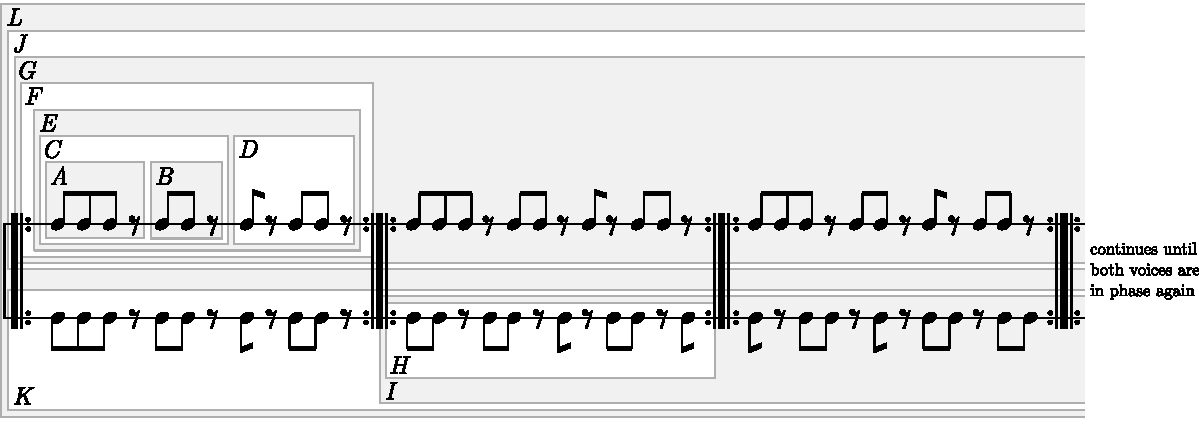
\includegraphics[width=\linewidth]{figs/clapping_patterns.pdf}
  \caption{Structures of S. Reich's \emph{Clapping Music}.}
  \label{fig:boat1}
\end{figure}

{\color{red}

Figure \ref{fig:boat1} is here.

}

\subsection{Code and interface for the experiments}

{\color{red}

[manual coding to extract procedural and extendable knowledge]\cite{Hofmann2015} 

}

\subsection{Decoded genotype: a procedural function tree of the piece}

\begin{lstlisting}[float][language=Java, caption=A possible decoded genotype for S. Reich's \emph{Clapping Music}]
s2V(                           // score L: joins the 2 voices vertically
  vSlice(                      // voice J: slices last cycle because of phase lag
    vRepeatV(                  // phase G: F 13 times
      vRepeatV(                // cycle F: E 8 times 
        vConcatV(              // pattern E: C + D
          vConcatV(            // motif C: A + B
            vMotifLoop(        // core motif A: 3 8th-notes and a silence
              ln(1/8),         // note values
              lm(65),          // pitch (irrelevant for this piece)
              la(50),          // articulation
              li(60,60,90,0)), // intensities (last note louder for clarity) 
            vSlice(            // motif B: A with 1st note sliced
              vAutoref(0),
              q(1))),
          vSlice(              // motif D: C with first two notes sliced
            vAutoref(3),
            q(2))),
        q(8)),
      q(13)),
    q(-12)),
  vConcatV(                    // voice K: F + H
    vAutoref(7),
    vRepeatV(                  // phase I: H 12 times 
      vSlice(                  // cycle H: cycle F with 1st note sliced
        vAutoref(10),
        q(1)),
      q(12))))
\end{lstlisting}

\begin{figure}
  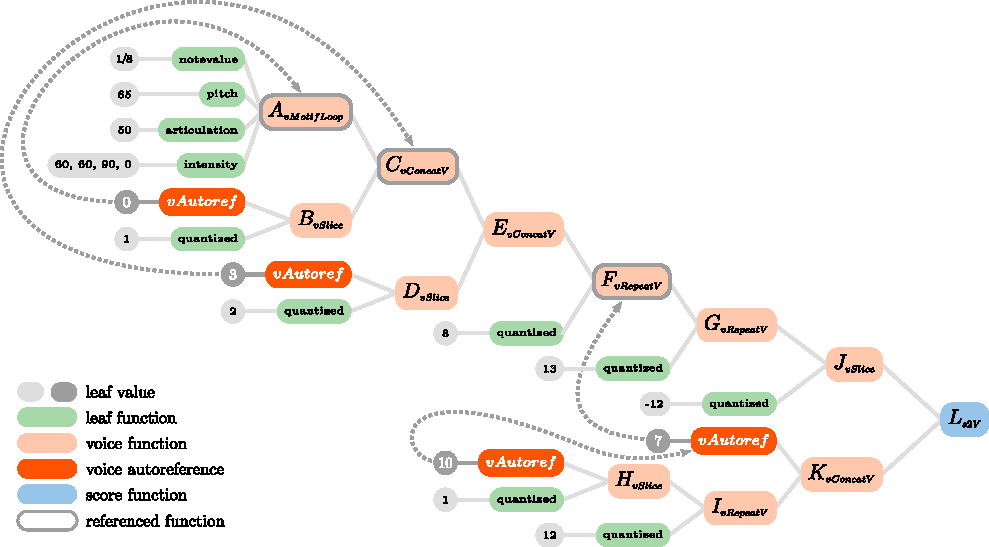
\includegraphics[width=\linewidth]{figs/clapping_tree_graph_colours_code.pdf}
  \caption{Structures of S. Reich's \emph{Clapping Music}.}
  \label{fig:boat2}
\end{figure}



\begin{figure}
\begin{center}
  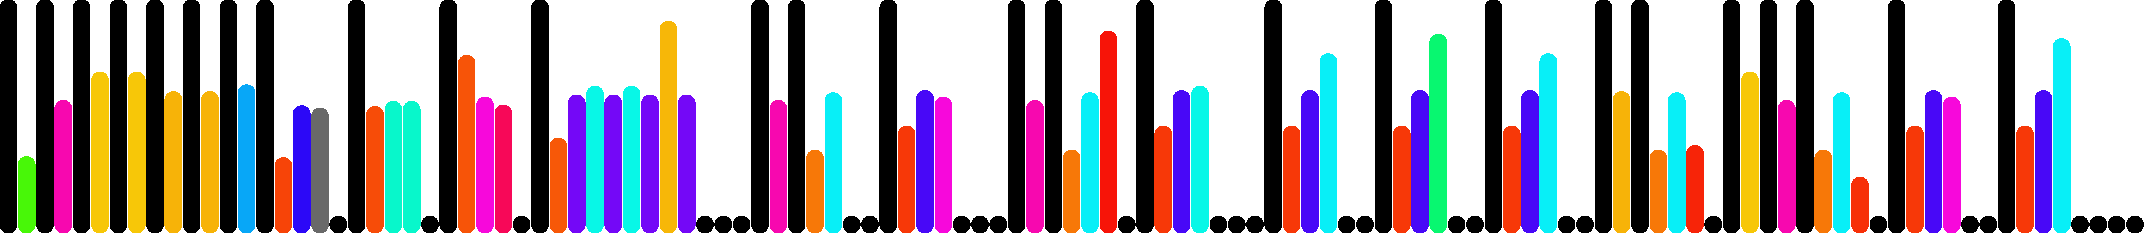
\includegraphics[width=11cm]{figs/clappingVisualized.pdf}
\end{center}  
  \caption{Structures of S. Reich's \emph{Clapping Music}.}
  \label{fig:boat3}
\end{figure}



{\small \begin{enumerate}[start=0]
\item \begin{verbatim}
"vMotifLoop(ln(0.125),lm(65),la(49),li(60,60,90,0))"
\end{verbatim}
\item \begin{verbatim}
"vAutoref(0)"
\end{verbatim}
\item \begin{verbatim}
"vSlice(vAutoref(0),q(1))"
\end{verbatim}
\item \begin{verbatim}
"vConcatV(vMotifLoop(ln(0.125),lm(65),la(49),li(60,60,90,0)),vSlice(vAutoref(0),q(1)))"
\end{verbatim}
\item \begin{verbatim}
"vAutoref(3)"
\end{verbatim}
\item \begin{verbatim}
"vSlice(vAutoref(3),q(2))"
\end{verbatim}
\item \begin{verbatim}
"vConcatV(vConcatV(vMotifLoop(ln(0.125),lm(65),la(49),li(60,60,90,0)),vSlice(vAutoref(0),
q(1))),vSlice(vAutoref(3),q(2)))"
\end{verbatim}
\item \begin{verbatim}
"vRepeatV(vConcatV(vConcatV(vMotifLoop(ln(0.125),lm(65),la(49),li(60,60,90,0)),vSlice(
vAutoref(0),q(1))),vSlice(vAutoref(3),q(2))),q(8))"
\end{verbatim}
\item \begin{verbatim}
"vRepeatV(vRepeatV(vConcatV(vConcatV(vMotifLoop(ln(0.125),lm(65),la(49),li(60,60,90,0)),
vSlice(vAutoref(0),q(1))),vSlice(vAutoref(3),q(2))),q(8)),q(13))"
\end{verbatim}
\item \begin{verbatim}
"vSlice(vRepeatV(vRepeatV(vConcatV(vConcatV(vMotifLoop(ln(0.125),lm(65),la(49),li(60,60,
90,0)),vSlice(vAutoref(0),q(1))),vSlice(vAutoref(3),q(2))),q(8)),q(13)),q(-12))"
\end{verbatim}
\item \begin{verbatim}
"vAutoref(7)"
\end{verbatim}
\item \begin{verbatim}
"vAutoref(10)"
\end{verbatim}
\item \begin{verbatim}
"vSlice(vAutoref(10),q(1))"
\end{verbatim}
\item \begin{verbatim}
"vRepeatV(vSlice(vAutoref(10),q(1)),q(12))"
\end{verbatim}
\item \begin{verbatim}
"vConcatV(vAutoref(7),vRepeatV(vSlice(vAutoref(10),q(1)),q(12)))"
\end{verbatim}
\end{enumerate}}



Extrapolacion de estructuras y variantes:

{\small \begin{verbatim}sClappingMusic (1/8,65,50,(60,60,90,0),1,2,8,13,-12,1,12)\end{verbatim}}  

 

\subsection{Encoded genotype: an abstract representation of compositional processes}

\begin{lstlisting}[language=Java, caption=Encoded genotype for S. Reich's \emph{Clapping Music}]
[1, 0.275535, 1, 0.534808, 1, 0.665631, 1, 0.665631, 1, 0.575462, 1, 0.575462, 1, 0.606798, 1, 0.27051, 0.51, 0.5, 0, 1, 0.506578, 0.53, 0.53, 0, 1, 0.742646, 0.55, 0.51346, 0, 1, 0.36068, 0.56, 0.6, 0.56, 0.6, 0.56, 0.9, 0.56, 0, 0, 0, 1, 0.534808, 1, 0.304952, 0.57, 0, 0, 1, 0.416408, 0.58, 0.55, 0, 0, 0, 1, 0.534808, 1, 0.304952, 0.57, 0.854102, 0, 1, 0.416408, 0.58, 0.6, 0, 0, 0, 1, 0.416408, 0.58, 0.75, 0, 0, 1, 0.416408, 0.58, 0.84, 0, 0, 1, 0.416408, 0.58, 0.75, 0, 0, 1, 0.575462, 1, 0.304952, 0.57, 0.326238, 0, 1, 0.665631, 1, 0.534808, 1, 0.304952, 0.57, 0.18034, 0, 1, 0.416408, 0.58, 0.55, 0, 0, 1, 0.416408, 0.58, 0.82, 0, 0, 0, 0]
\end{lstlisting}

\subsection{Encoded phenotype and possible outputs}

{\color{red}


\begin{itemize}



\item Un ejemplo clasico con varias voces y conteniendo armonia, dinamica y articulacion
\item Modularidad y posibilidad de manipulacion manual
\item Ejemplos basicos de tecnicas habituales en CAC (movimiento browniano,
\item Handling of recursive techniques (fibonacci, y extension del modelo a expresiones matematicas complejas)
\item Puentes entra la notacion tradicional, la sintesis de sonido y la espacializacion
\item Multimedia
\end{itemize}

}



%------------------------------------------------
\section{Evaluation and evolution}

\begin{samepage}
\begin{quotation}
\textsl{Edward Fredkin suggested to me the theory that listening to music might exercise some innate map-making mechanism in the brain. When I mentioned the puzzle of music's repetitiousness, he compared it to the way rodents explore new places: first they go one way a little, then back to home. They do it again a few times, then go a little farther. They try small digressions, but frequently return to base. Both people and mice explore new territories that way, making mental maps lest they get lost. Music might portray this building process, or even exercise those very parts of the mind.}

---Marvin Minsky \cite{Minsky1981}\end{quotation}
\end{samepage}


{\color{red}


\cite{Biles94genjam} para el problema del ?fitness bottleneck? con la eval. humana


\cite{Burton1999}  -> IMPORTANTE distincion entre Genetic Programming and Gen. Algorithms: 'An overview of earlier
studies in EC for musical composition is offered in [12], determining that Ge-
netic Programming (GP) methods perform better than those that use Genetic
Algorithms (GA). This may be unsurprising as GP methods use a tree-based
structure whereas GAs are limited to a linear string in their representation.
Hence, GP can represent more complex representations and operations | some-
thing that would be very useful in representing music.'





\cite{LimitHuman} -> The evolution of a population offers so much scope and possibility
that it is reminiscent of the music creation process a solution is not linearly
determined but instead emerges from a 
uid, incremental process.



\cite{DBLP:journals/aim/Minsky82} - > interesantes perspectivas de la
evaluacion, relacionadas con los prejuicios apuntados por Minsky

Citar \cite{BurtonHybrid} para
-> Ejemplo de sistema basado en programacion textual, para introduccion manual de expresiones complejas
	-> A menudo son sistemas creados por los propios compositores como medio de extender su estilo
	
	
Buscar donde meter el asunto de la hibridacion
Otro ejemplo de hibrido -> \cite{crawford2015algorithmic}

El texto de \cite{Papadopoulos98agenetic}
segun Mantaras, usan fitness basado en contorno, intervalica, y otras cuestiones cuantificables

}

When modeling artistic creativity with algorithms, probably the most evasive issue to address is programming fitness functions. By definition, the assessment of a piece of art can only be made from a subjective point of view, since the goal of art is to provoke inner and personal reactions. These individual responses are very dependent on cultural and social context. However, provided enough data some predictions can be made about the expected rating for a new piece.

In GenoMus, we divide evaluation of each specimen in two categories:

\begin{itemize}
\item Autoanalytic profile: objective analysis of a set of musical features, such as variability, rhythmic complelxity, tonal stability, global dissonance index, level of inner autoreference, etc. 
\item Human evaluations: subjective ratings made by human users, attending to aesthetic value, originality, mood and emotional intensity. This informations are stored individually and together as global statistics.

\end{itemize}

The self-analysis contained in every specimen allows to measure distance and similaritiy to  
other specimens, as well as to classify results and to drive evolution processes.

Defining how to evaluate and select results is now the most creative effort, and can be identified with the act of composition itself, since composing music is ultimately making choices. 


{\color{red}


\begin{itemize}
\item Esta propuesta de gramatica posibilita la implementacion y competencia de diferentes sistemas de evaluacion
\item Design of evaluation methods as the crucial act of composition
\item Objective vs. subjective evaluation
\item What to learn?
\item Evolutionary paradigm as the most promising
\end{itemize}


}


\subsection{Evolutionary paradigm}

Determining how to evolve and mutate an specimen towards a best version is crucial question too. Starting from a simple motif, endless evolution paths can lead to satisfying results based on heuristic approaches, using accumulated knowledge from examples, human ratings and automatic self-analysis.

The GenoMus grammar is designed to favor the broadest diversity of combinations and transformations. Genetic algorithms are suitable for the automation of an incremental exploration and selection of multiple ways. A GenoMus decoded genotype tree expression can be trasnformed using these methods:

\begin{itemize}
\item createGen
\item mutateLeaves
\item growTrunk
\item growBranch
\item insertBranch
\item flattenBranch
\item pruneBranch
\item splitGen

\end{itemize}

Approaches based on neural networks need a very controlled format of data and big training datasets. The encoded genotype format of GenoMus can represent any piece of music as a simple unidimensional sequence of normalized floats, which can be profitable for techniques as recurrent neural networks (ref. to LMSTD), able to learn patterns from sequential streams of data.


\subsection{Scalability}

{\color{gray}


\begin{itemize}
\item Como conjugar universalidad de las expresiones con optimizacion para tener los vectores codificados con mayores diferencias entre si.
\item Estrategias de caracterizacion de perfiles estilisticos
\item El problema del mapeo de funciones y su extensibilidad
\item Como establecer una base de datos de conocimiento
\item Metricas automatizadas de ciertos resultados
\end{itemize}

}


\subsection{Integrating traditional and contemporary techniques}

\subsection{Expanding our musical perception}


{\color{red}

\cite{quteprints6544} -> para afirmar que GenoMus reune diferentes paradigmas en sus arboles multicapa. Estos paradigmas segun el articulo son: Analytic, Transformational and Generative
}

{\color{gray} \textsl{[A genotype como un arbol multiagente, que puede incorporar nodos con funciones de todo tipo: analiticos, recursivos, de constraints, etc. Una vez se tiene un marco de funcion, todo puede caber en el arbol de procesos.]}}


{\color{red}

Justificar con \cite{LopezdeMantaras:2006:MMA:1565082.1565089}:
	-> 2: En los 50 era logico excliur la parte expresiva. Los modelos Markovianos son de resultados muy pobres. Ahora debe estar incluida?
IMPORTANTE:
	-> referencia a Minsky, que plantea la posibilidad de los multiagentes, que puedan actuar sobre bloques mayores de musica, y que sean a veces solo analiticos
	-> ?the rules dont make the music, it is the music that makes the rules?
	-> Truly creative! para el final
}


%------------------------------------------------
\section{Conclusions and ongoing work}

\begin{samepage}
\begin{quotation}
\textsl{A generation later, we should be experimenting on programs
that write better programs to replace themselves. Then
at last it will be clear how foolish was our first idea---that
never, by their nature, could machines create new things.}

---Marvin Minsky \cite{DBLP:journals/aim/Minsky82}
\end{quotation}
\end{samepage}

{\color{red}

\cite{Papadopoulos99aimethods} -> concluye que los avances prometedores vendran de la integracion de sistemas diferentes

De la referencia citada al principio \cite{LopezRincon2018}: ?Symbolic AI methods still have not enough rules therefore,
they hardcoded in limited database knowledge. This could be
extended with machine learning techniques but the lack of an
automatic evaluation method makes it difficult to solve.?

}


The artistic results of every algorithm designed for automated composition
are strongly constrained by their own representation
system of musical data. This paper presents GenoMus, a
framework for the exploration of artificial musical creativity
based on a generative grammar focused on the abstraction
of creative processes as a metalevel of compositional
tasks. We define musical genotypes as functional
nested expressions, and phenotypes as the pieces created
by evaluating these computable expressions. GenoMus' grammar is designed 
to ease the combination of fundamental procedures behind very different styles, ranging from basic to complex contemporary
techniques, particularly those able to produce rich
output from very simple recursive algorithms. At the same
time, maximal modularity is provided to simplify metaprogramming
routines to generate, assess, transform and categorize
the selected musical excerpts. The system is conceived
to maintain a long term interrelation with different
users achieving individual musical styles. This proposed
grammar can also be an analytic tool, from the point of
view of composition as computation, considering that the
best analysis of a piece is the shortest precise description.

{\color{gray}

Cuestiones interesantes: 
\begin{itemize}
\item ?Cuantas funciones primitivas son necesarias para generar musica en un determinado estilo? Hay innumerables expresiones funcionales diferentes que pueden generar la misma musica. Se puede deducir que la expresion funcional mas breve es el mejor analisis. Se pueden ver diferentes paradigmas de ensenanza/aprendizaje de la musica con estos modelos.
\item ?Como puede hacerse ingenieria inversa automatizada para extraer estructuras desde la musica?
\end{itemize}
}

%------------------------------------------------
\bibliographystyle{acm}  
\bibliography{references}  

\end{document}